\section{Вступление}

Photometric stereo — метод в компьютерном зрении для определения
нормалей поверхности объектов путем наблюдения за этим объектом
при различных условиях освещения. Он основан на том факте,
что количество света, отражаемого поверхностью, зависит от ориентации
поверхности относительно источника света и наблюдателя.

\begin{figure}[h]
  \centering
  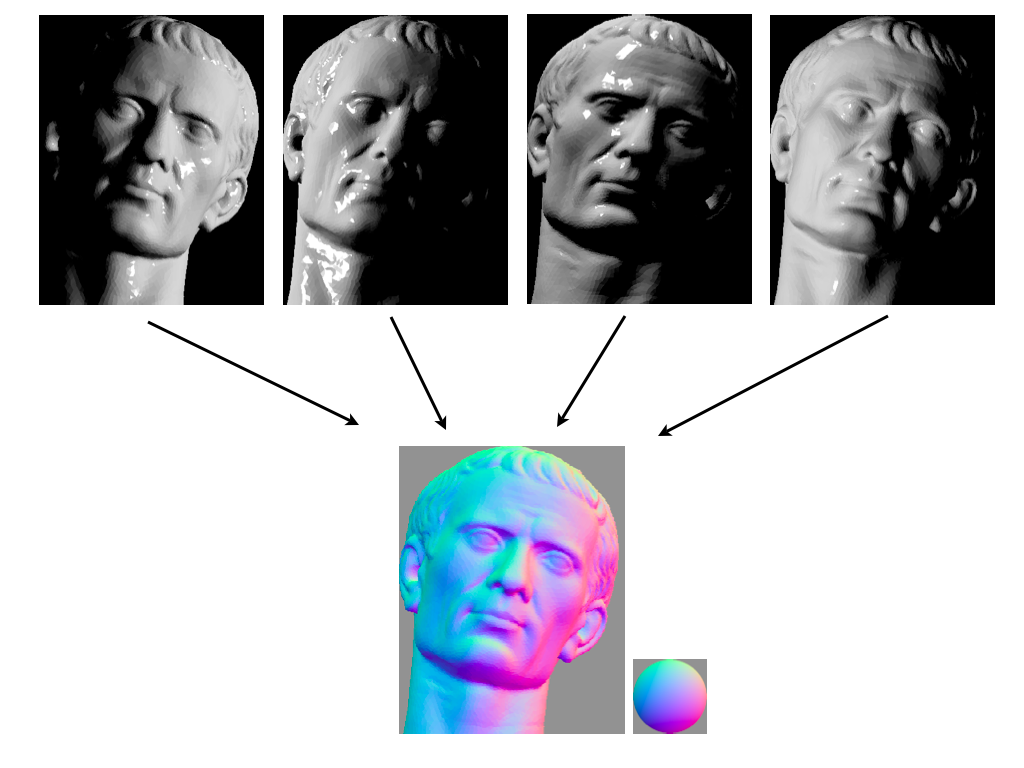
\includegraphics[scale=0.3]{tex/example.png}
\end{figure}

При использовании этого метода путем измерения количества света,
отраженного в камеру, пространство возможных ориентаций поверхности может
быть ограничено. Если объект наблюдается под достаточным количеством источников
света с разных углов, то ориентация поверхности может быть ограничена
до одной ориентации или даже получиться больше, чем необходимо.

Метод был впервые предложен в 1980 году Уодхэмом. Особый случай,
когда данные представлены одним изображением, известен как "shape from shading",
и был анализирован Б. К. П. Хорном в 1989 году. Расширенные методы фотометрического
стерео были разработаны для учета проецируемых теней и других
неоднородных условий освещения.

Однако, этот метод требует тщательного планирования и контроля эксперимента,
чтобы получить необходимое количество данных, и считается,
что он неэффективен для объектов с неоднородной поверхностью
и большим числом полостей. Тем не менее, photometric stereo все еще остается
важной технологией в области компьютерного зрения, особенно для задач
реконструкции трехмерных объектов.
